\documentclass{beamer}
\usepackage[utf8]{inputenc}
\usepackage{graphicx}

\usetheme{Madrid}
\usecolortheme{default}
\useinnertheme{circles}

\definecolor{Logo1}{rgb}{0.208, 0.2865, 0.373}
\definecolor{Logo2}{rgb}{0.000, 0.674, 0.863}

\setbeamercolor*{palette primary}{bg=Logo1, fg=white}
\setbeamercolor*{palette secondary}{bg=Logo2, fg=white}
\setbeamercolor*{palette tertiary}{bg=white, fg=Logo1}
\setbeamercolor*{palette quaternary}{bg=Logo1,fg=white}
\setbeamercolor{structure}{fg=Logo1} % itemize, enumerate, etc
\setbeamercolor{section in toc}{fg=Logo1} % TOC sections

%------------------------------------------------------------
%This block of code defines the information to appear in the
%Title page
\title{Introduction to Depth Estimation}
\subtitle{Pre-Machine Learning Era}

\author{Chinchuthakun Worameth}

\institute[]{
  Department of Transdisciplinary Science and Engineering\\
  Tokyo Institute of Technology
}

\date{\today}


%\logo{
\includegraphics[height=.5cm]{logo-footer.png}}

%End of title page configuration block
%------------------------------------------------------------



%------------------------------------------------------------
%The next block of commands puts the table of contents at the 
%beginning of each section and highlights the current section:

% \AtBeginSection[]
% {
%   \begin{frame}
%     \frametitle{Table of Contents}
%     \tableofcontents[currentsection]
%   \end{frame}
% }
%------------------------------------------------------------


\begin{document}

%The next statement creates the title page.
\frame{\titlepage}


%---------------------------------------------------------
%This block of code is for the table of contents after
%the title page
\begin{frame}
\frametitle{Table of Contents}
\tableofcontents
\end{frame}
%---------------------------------------------------------

\section{Definition}

%---------------------------------------------------------
%Changing visivility of the text
\begin{frame}{What is depth estimation?}
A task of predicting depth information/generating a corresponding \textbf{depth map} from images. 
\bigskip
\begin{columns}
    \begin{column}{.45\linewidth}\centering
    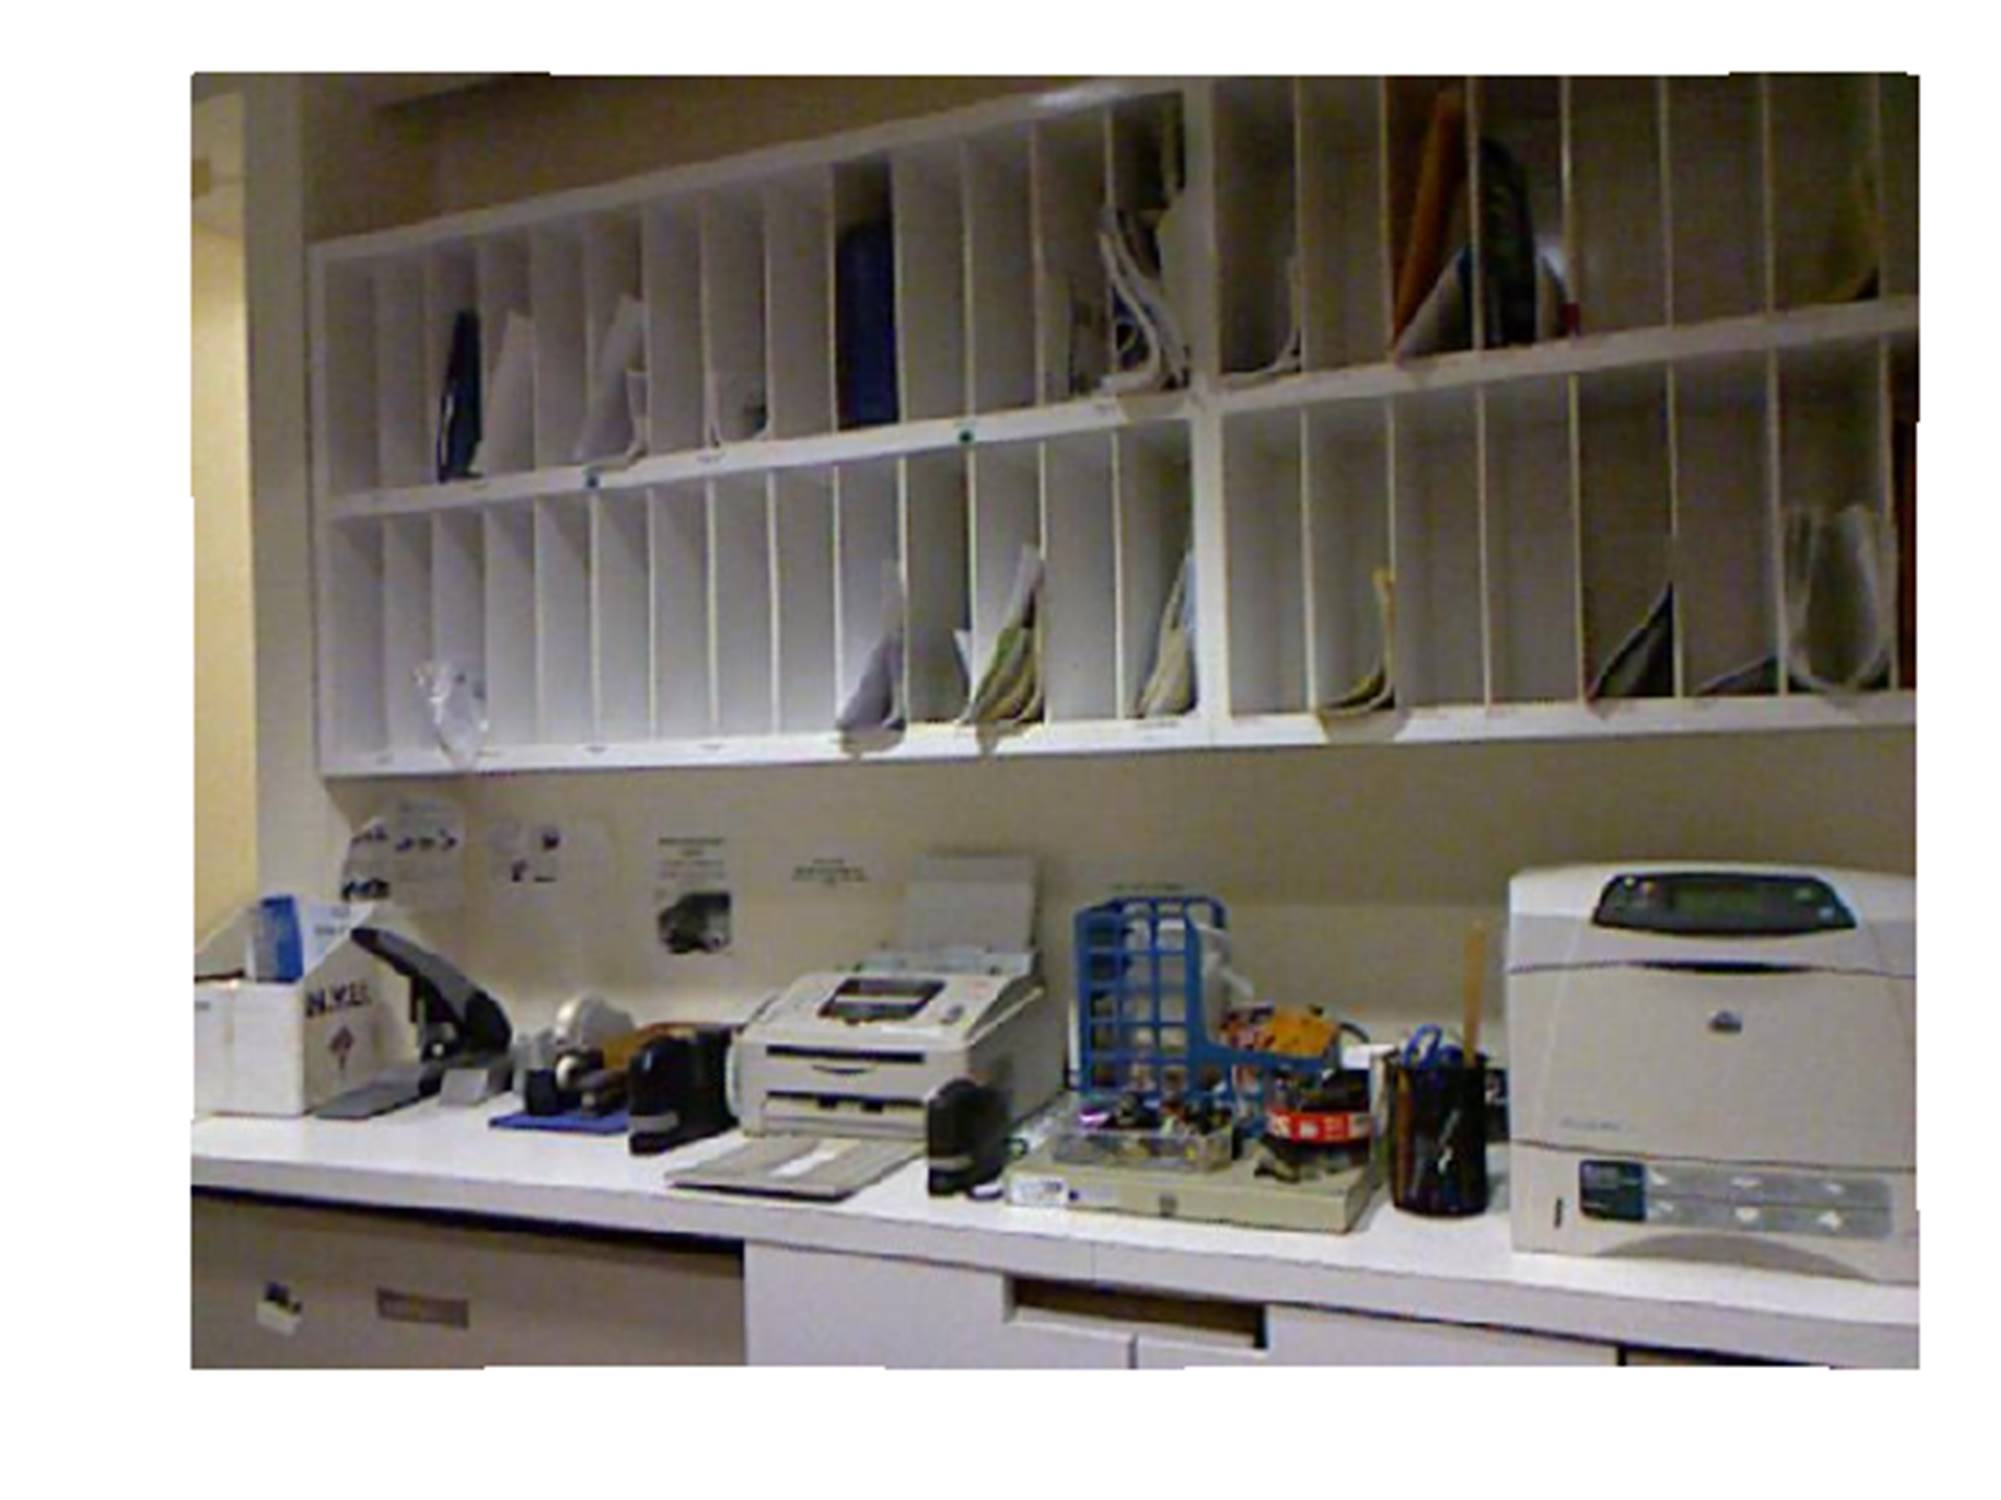
\includegraphics[width=5.3cm]{depthmap_real.jpg}\par
    Raw image \cite{chaijirawiwat_monocular_2019}
    \end{column}
    \begin{column}{.45\linewidth}\centering
    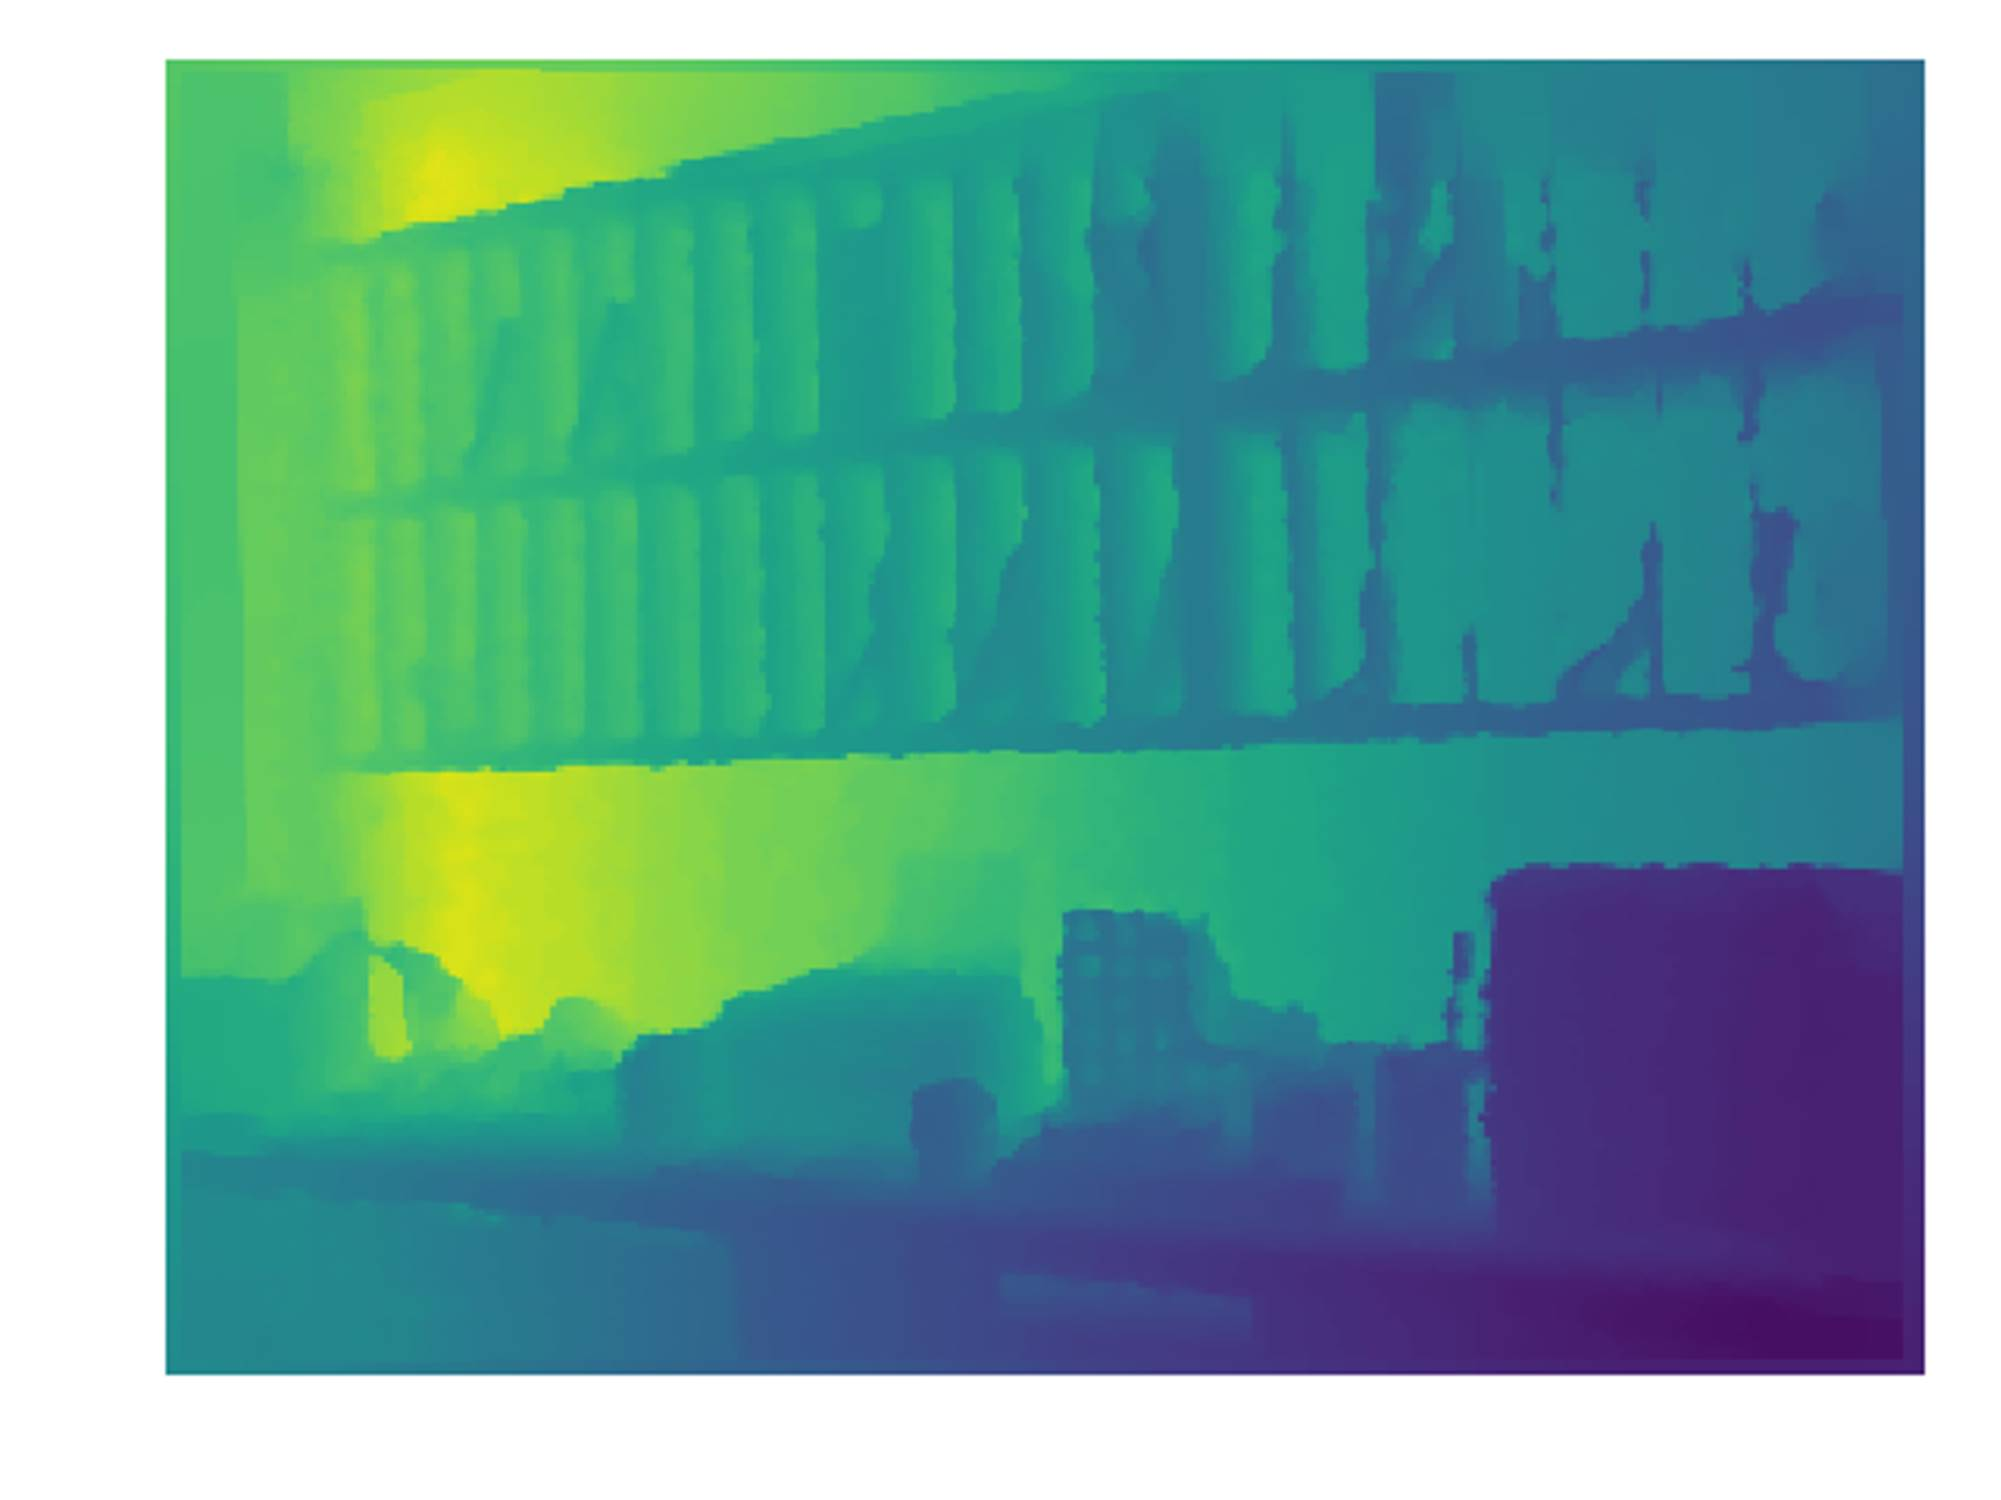
\includegraphics[width=5.3cm]{depthmap_depth.jpg}\par
    Depth map \cite{chaijirawiwat_monocular_2019}
    \end{column}
\end{columns}
\end{frame}

\begin{frame}{What is depth estimation? (con't)}
Approaches can be classified into:
\begin{itemize}
    \item \textbf{Active}: Emit waves to the scene and measure the time taken by it, e.g. \textbf{Time of flight (ToF)}.
    $$d=\frac{ct}{2}$$
    
    \item \textbf{Passive}: Measure distance by using image(s). Trading off between accuracy and processing time.
    \begin{itemize}
        \item \textbf{Monocular}: Single image or video sequence.
        \item \textbf{Stereo}: 2 images
        \item \textbf{Multiview}: $>2$ images
    \end{itemize}
\end{itemize}
\end{frame}

\section{Pinhole camera model}
\begin{frame}{Pinhole camera model}
    \begin{itemize}
        \item Project points in \textbf{real world coordinate} to \textbf{image coordinate}
        \item Can be defined by intrinsic parameters: \textbf{focal length $f$}, \textbf{principal point offset $(x_0,y_0)$}, and \textbf{axis skew $s$}.
    \end{itemize}
    \bigskip
    \begin{columns}
        \begin{column}{.4\linewidth}\centering
        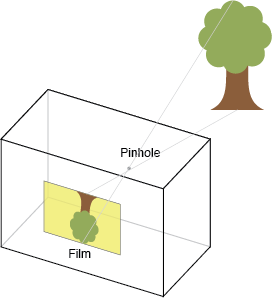
\includegraphics[width=3.5cm]{pinhole_overview.png}\par 
        Overview \cite{noauthor_perspective_nodate}
        \end{column}
        \begin{column}{.4\linewidth}\centering
        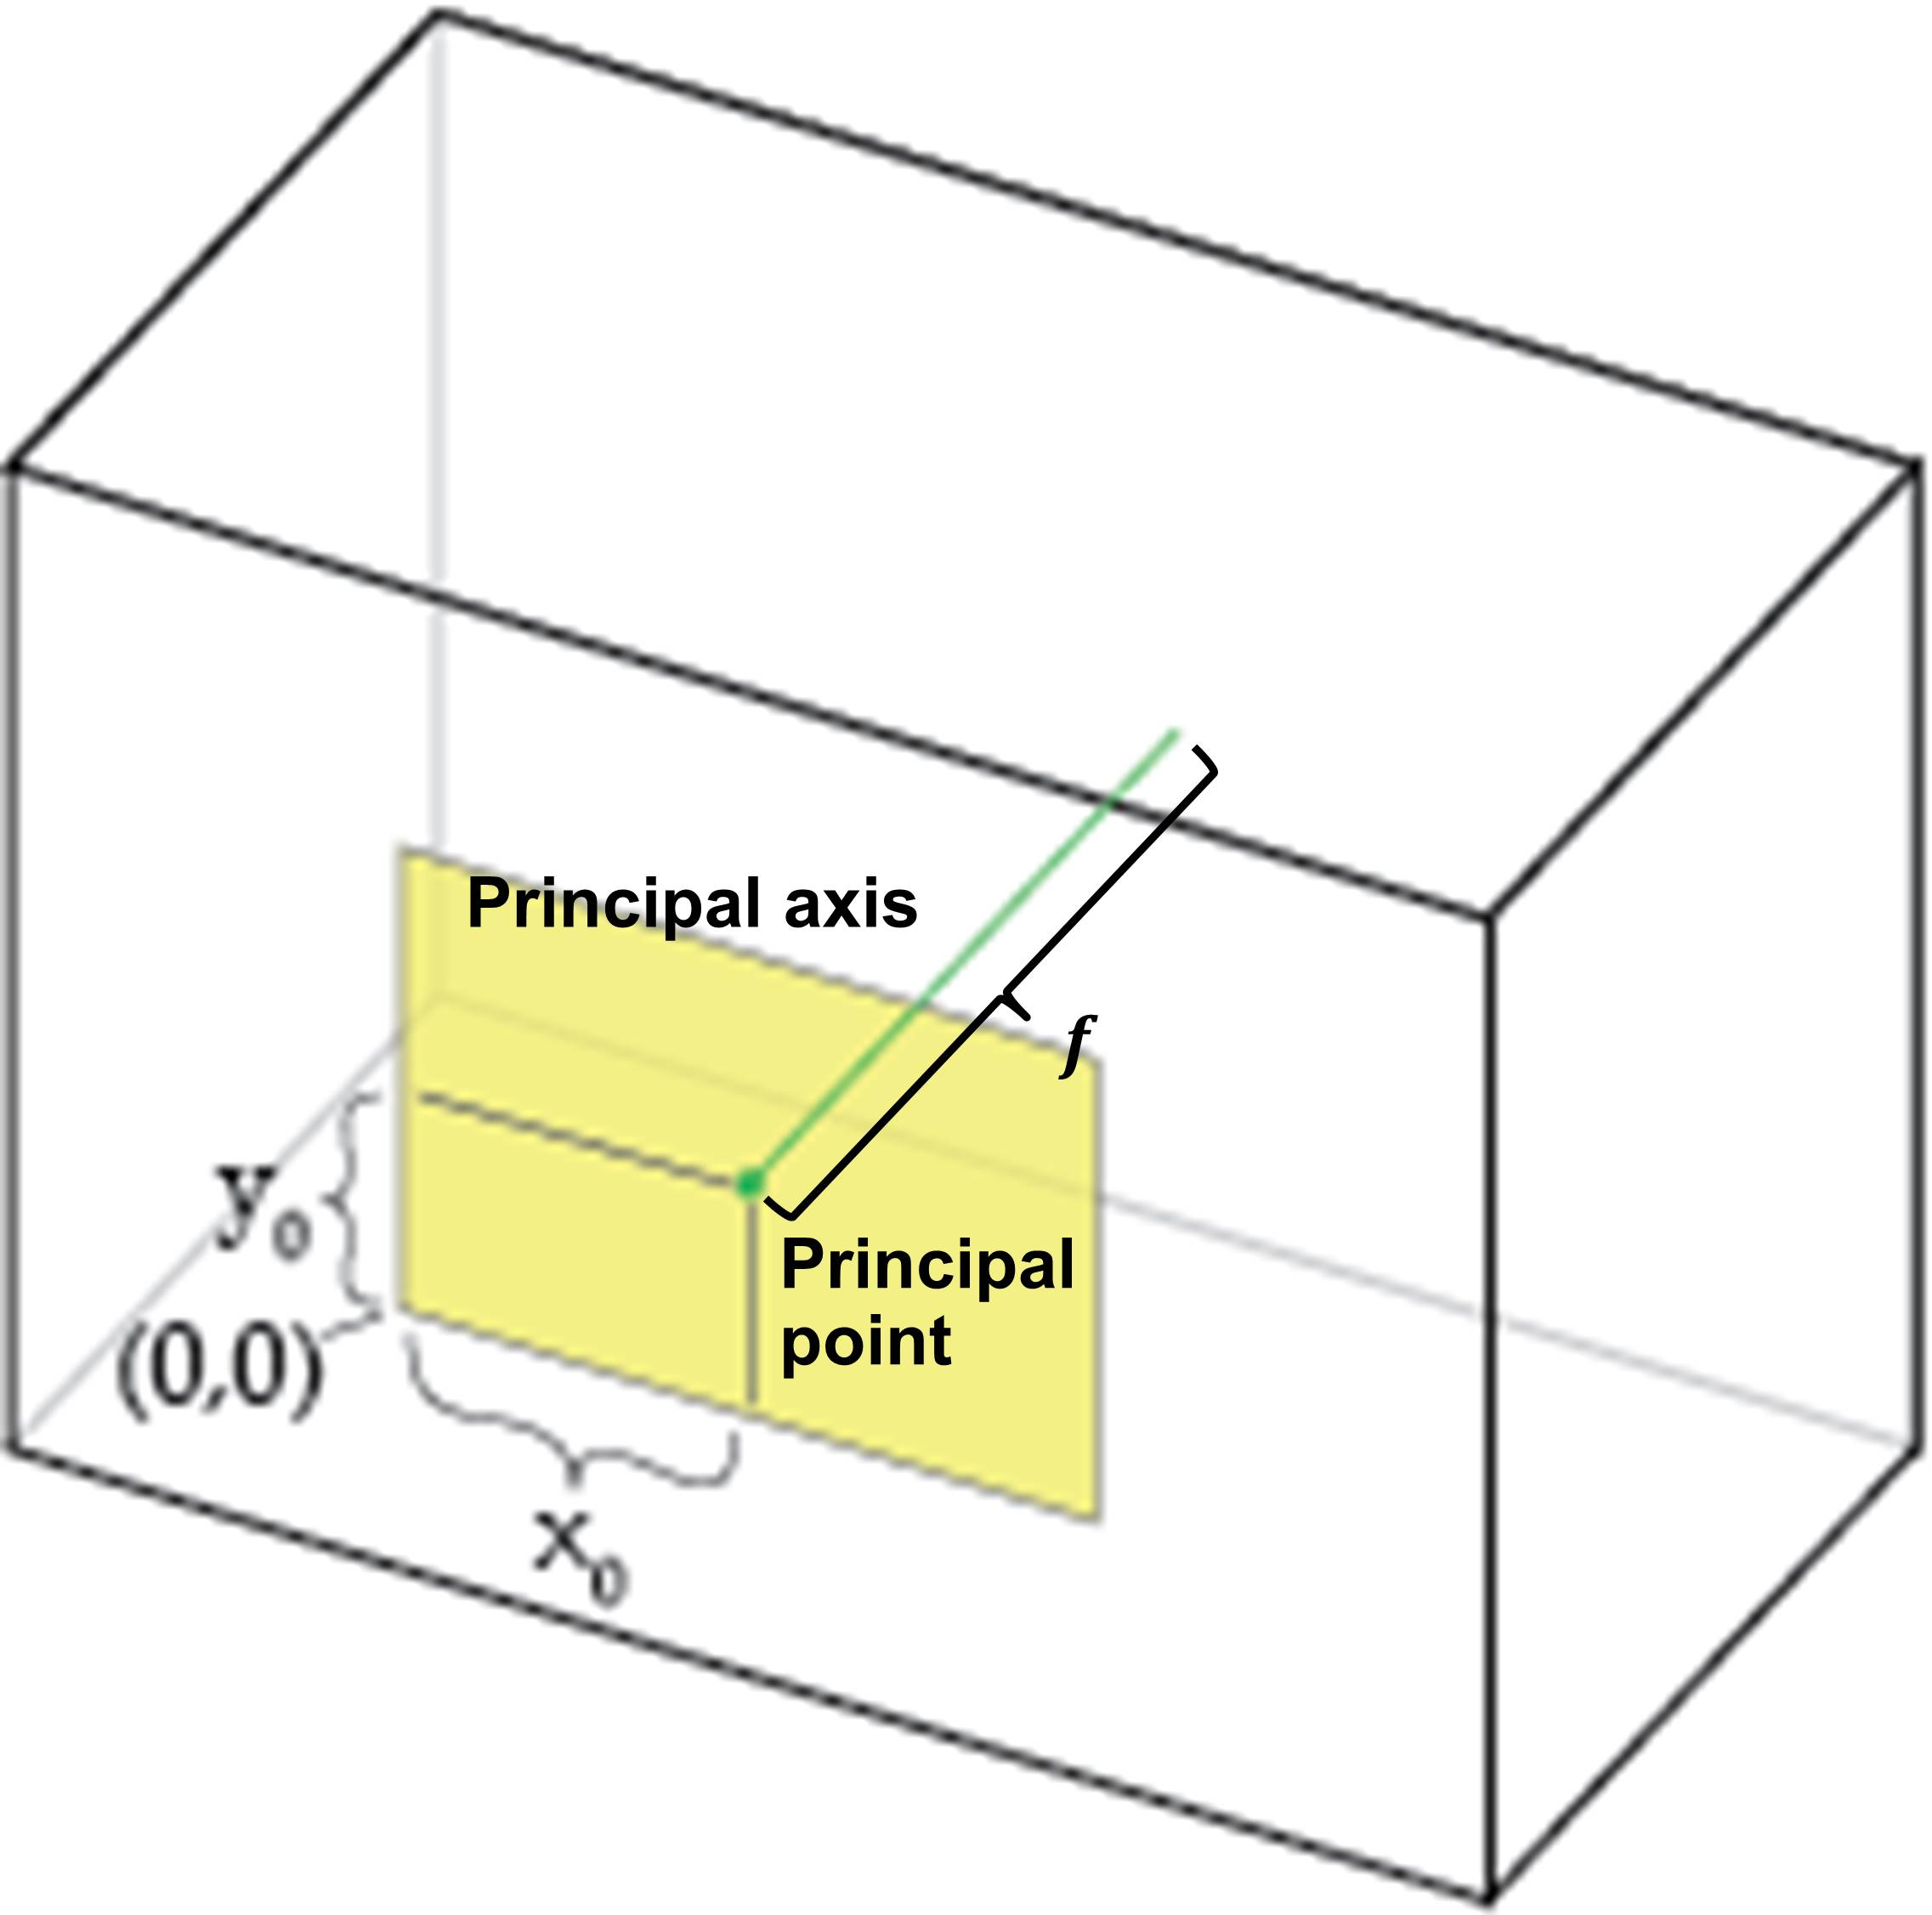
\includegraphics[width=3.5cm]{pinhole_description_mod.jpg}\par 
        Intrinsic parameters \cite{noauthor_perspective_nodate}
        \end{column}
    \end{columns}
\end{frame}

\begin{frame}{Pinhole camera model (con't)}
    \begin{columns}
        \column{0.5\textwidth}
        \textbf{Intrinsic/Calibration matrix}
        $$x=KX, K=\begin{bmatrix}
        f & s & x_0\\
        0 & af & y_0\\
        0 & 0 & 1
        \end{bmatrix}$$
        
        \column{0.5\textwidth}
        Assume $a=1$ and $s=0$, by defining image coordinate as below, we have
        $$x=f\frac{X}{Z} \text{ and } y=f\frac{Y}{Z}$$
    \end{columns}
    \smallskip
    \begin{center}
        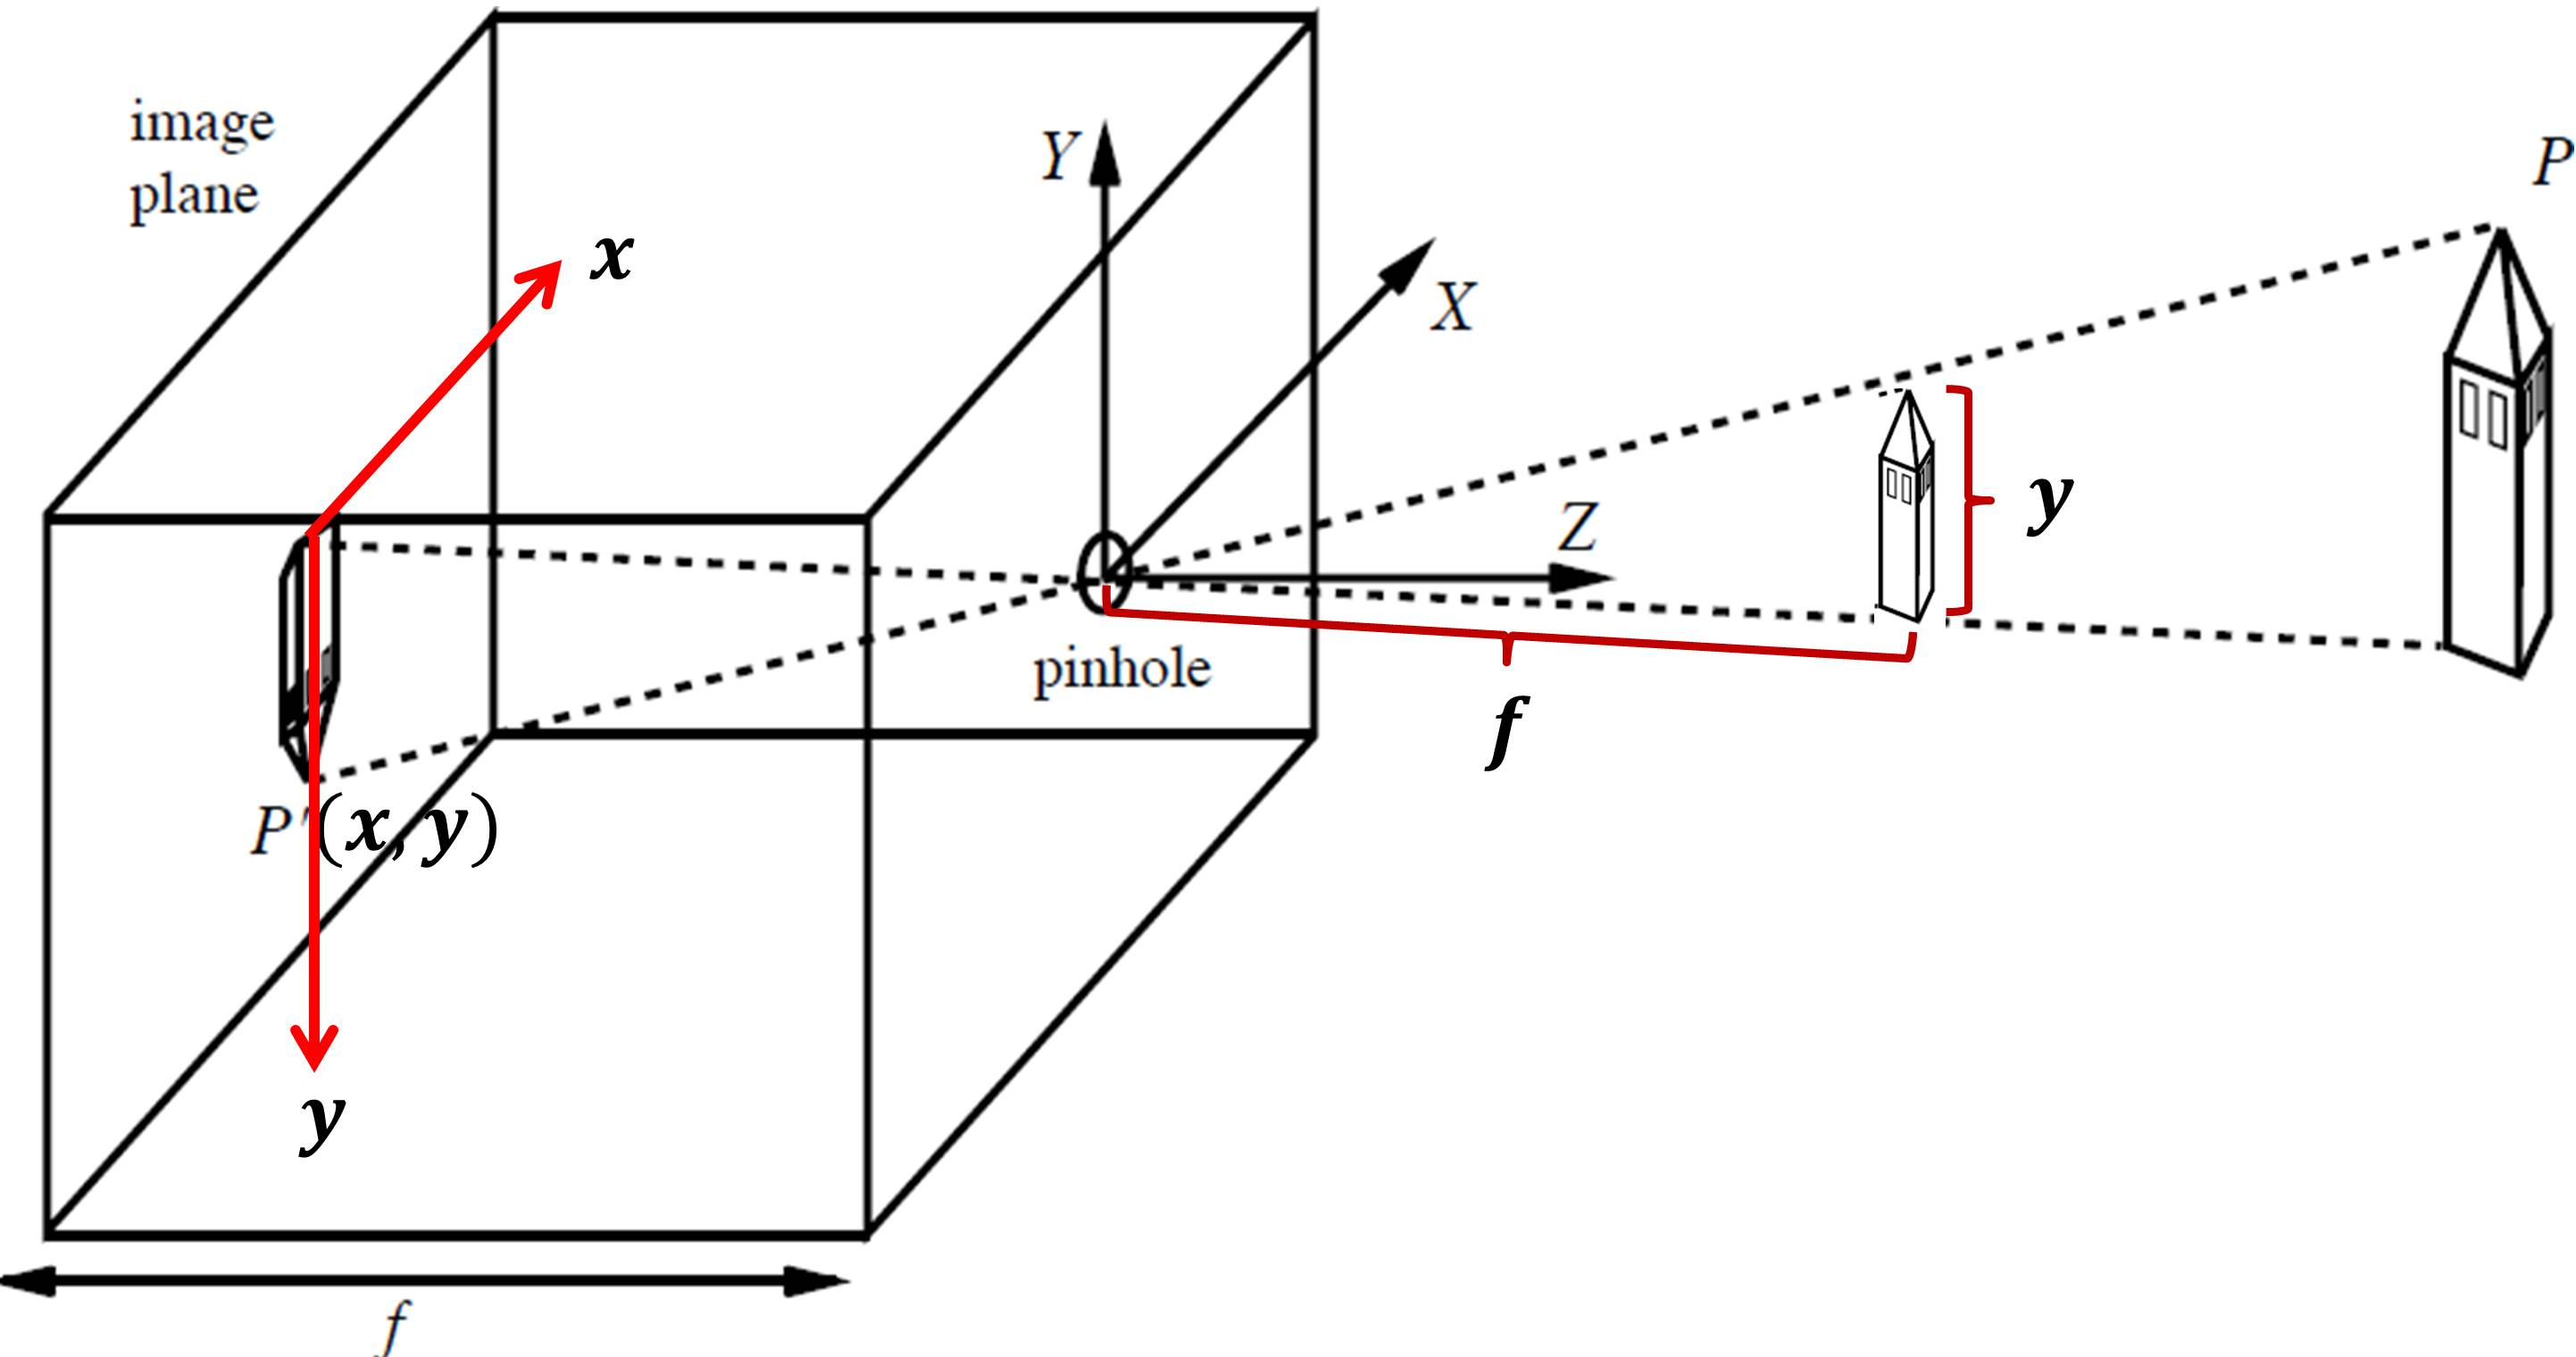
\includegraphics[width=8cm]{pinhole_derive.jpg}
        \par Image from \cite{noauthor_cs280:_nodate}
    \end{center}
\end{frame}

\begin{frame}{Pinhole camera model (con't)}
    We also need \textbf{Extrinsic matrix $[R \lvert t]$} because we need to consider the position of camera in the real world. Therefore, we can transform real world coordinate $P$ to image coordinate $p$ by using \textbf{camera matrix} $P$
    $$x=PX, P=K[R\lvert t]$$
    \begin{center}
        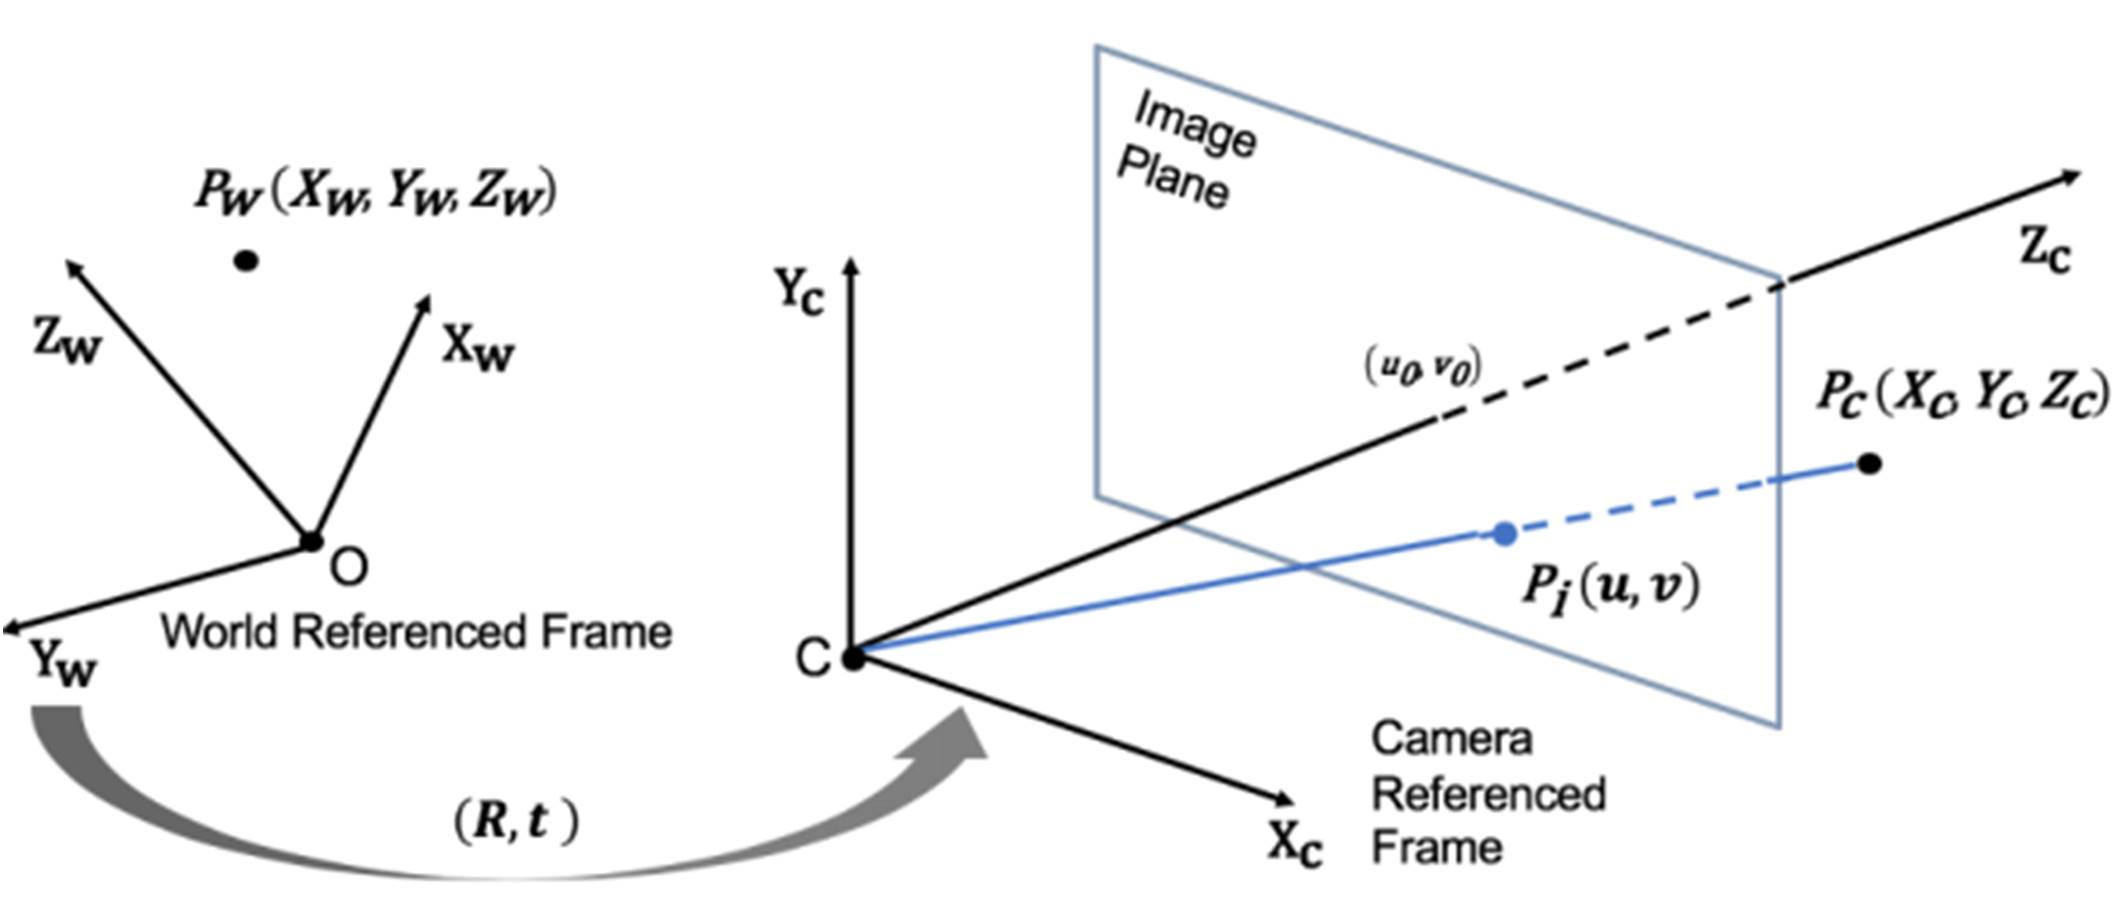
\includegraphics[width=8cm]{pinhole_extrinsic.jpg}
    \end{center}
\end{frame}

\section{Epipolar Geometry}
\begin{frame}{Epipolar Geometry}
    Geometry relationship of a scene from two points of view, shifted by $[R \lvert t]$
    \begin{itemize}
        \item \textbf{Epipolar plane}
        \item \textbf{Base line}: $\overline{C_LC_R}$
        \item \textbf{Epipole}: $e_L$ and $e_R$
        \item \textbf{Epipolar line}: $\overline{p_Le_L}$ and $\overline{p_Re_R}$
    \end{itemize}
    \begin{center}
        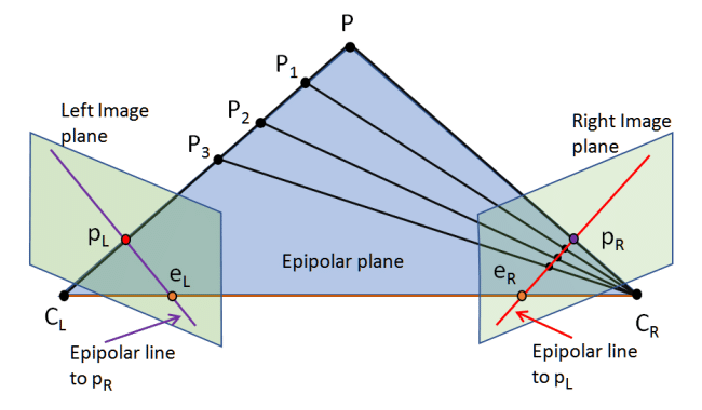
\includegraphics[width=7cm]{epipolar.JPG}
    \end{center}
\end{frame}

\begin{frame}{Epipolar Geometry (con't)}
    \textbf{Epipolar constraints}: Corresponding points (sometimes called \textbf{conjugate pair pixels}) must be observed on the same epipolar line.
    \begin{center}
        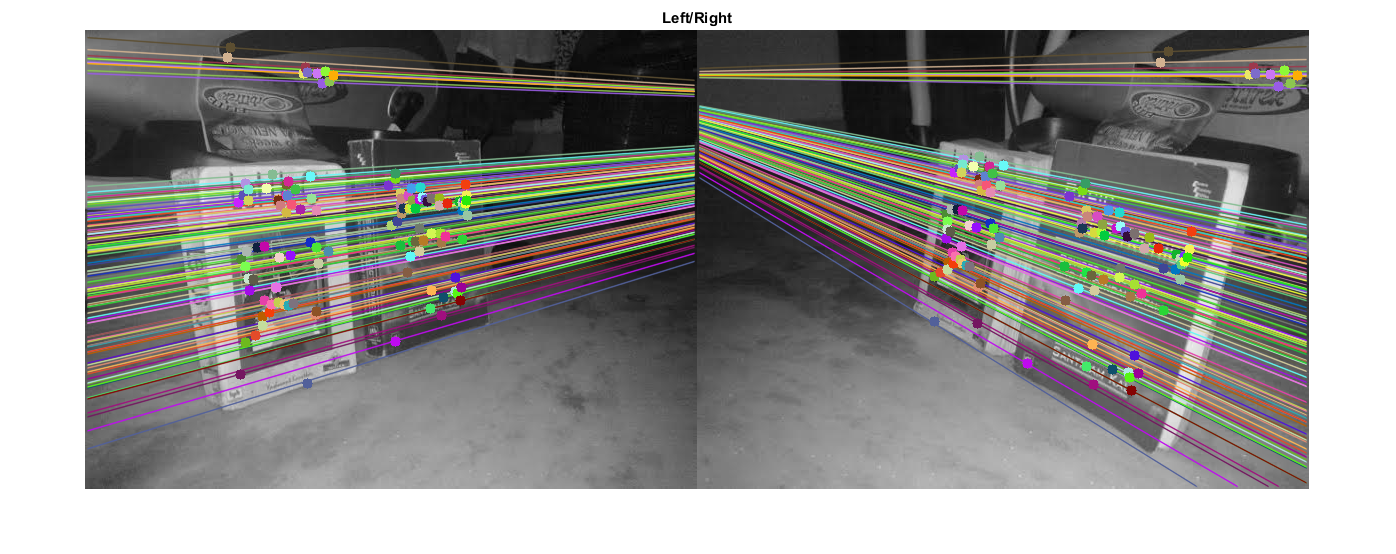
\includegraphics[width=12cm]{epipolar_demo1.png}
        \par Image from \cite{noauthor_epipolar_2017}
    \end{center}
\end{frame}

\section{Depth map}
\begin{frame}{How to get depth map?}
    \begin{enumerate}
        \item \textbf{Camera calibration}: determining camera matrix for each camera
        \begin{itemize}
            \item \textbf{Zhang's algorithm} \cite{zhang_flexible_2000} can recover parameters by using $>=2$ images of planar calibration objects, e.g. chess board, in different orientations.
        \end{itemize}
        \item \textbf{Image rectification}: recovering a simpler and more linear image from raw image
        \item \textbf{Image matching}: generating \textbf{disparity map}
        \item \textbf{Depth estimation}: calculating depth map from disparity map
    \end{enumerate}
\end{frame}

\begin{frame}{Image rectification}
    One simple method from \cite{fusiello_compact_2000} is shown below.
    \begin{columns}
        \begin{column}{.3\linewidth}\centering
        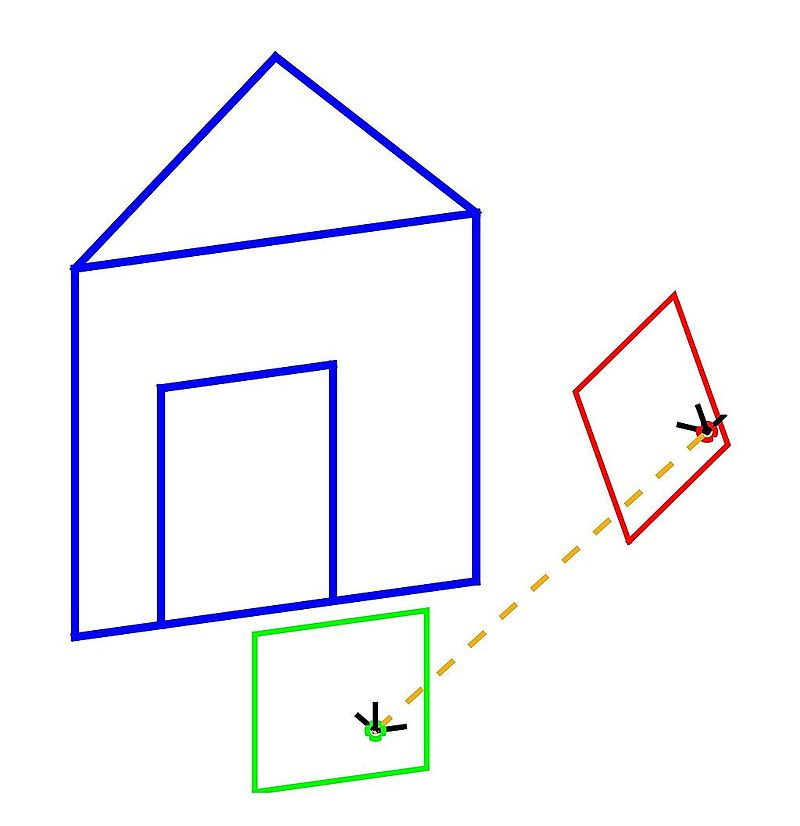
\includegraphics[width=5cm]{image_rectification_1.jpg}
        \end{column}
        \begin{column}{.6\linewidth}\centering
        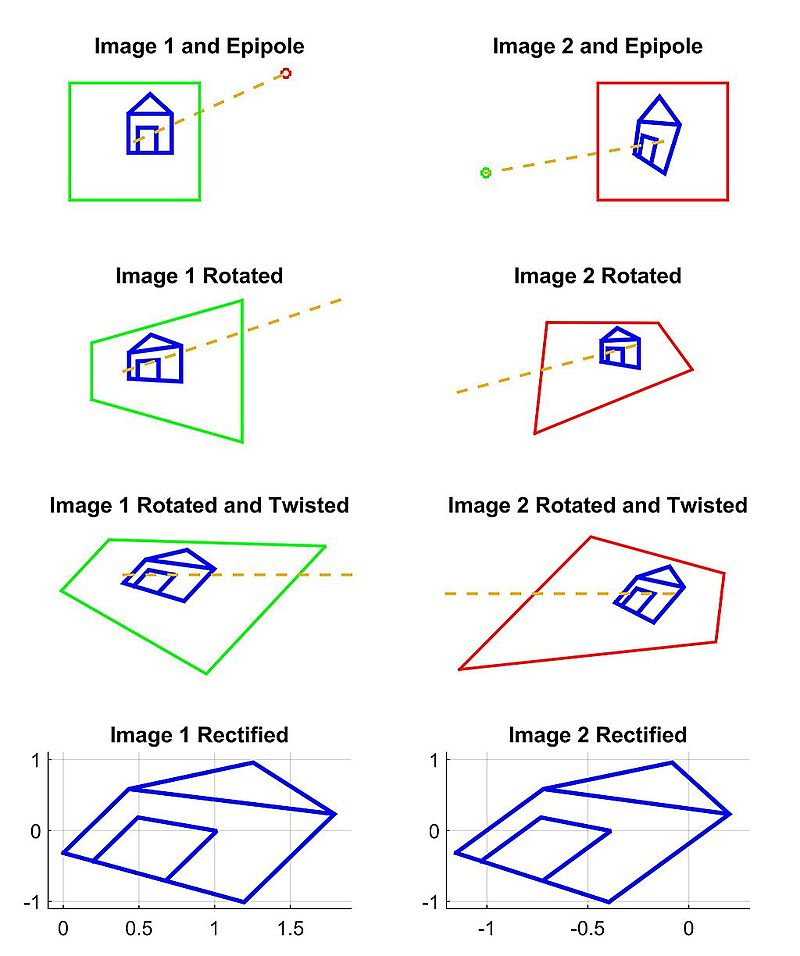
\includegraphics[width=5.5cm]{image_rectification_2.jpg}
        \end{column}
    \end{columns}
\end{frame}

\begin{frame}{Image matching: Block matching}
    One of the most intuitive method is \textbf{Block matching}. We call $d$ a \textbf{disparity} of image patch centered at $(u,v)$.
    \smallskip
    \begin{center}
        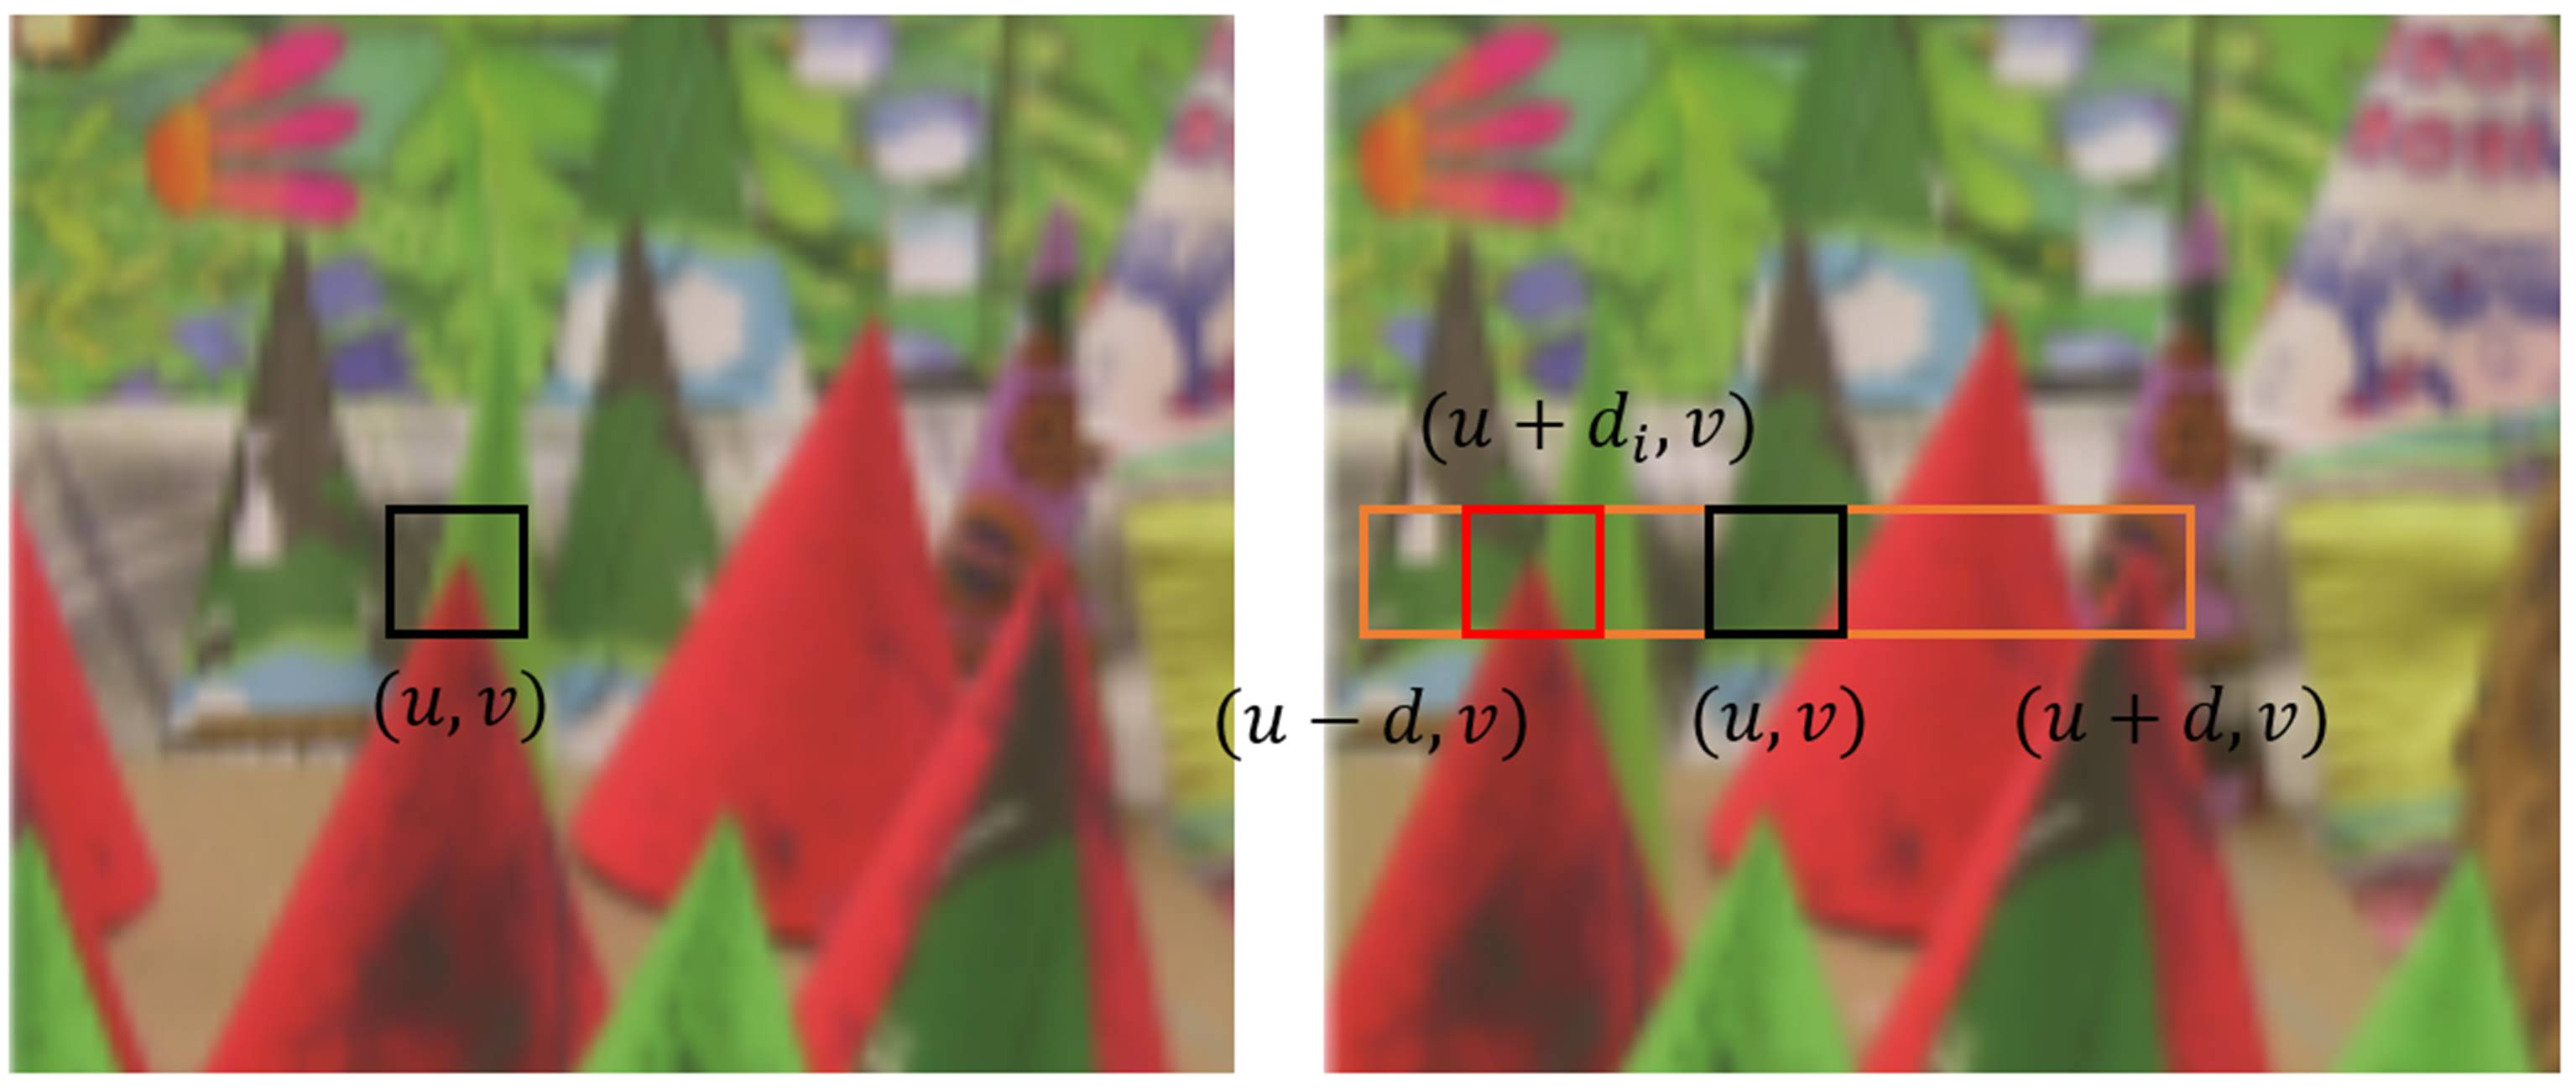
\includegraphics[width=10cm]{block_matching.jpg}
    \end{center}
    How to compare similarity between 2 image patches?
\end{frame}

\begin{frame}{Image matching: Block matching (con't)}
    \begin{itemize}
        \item \textbf{Correlation}: Normalized Cross-Correlation (NCC)
        $$C_{NCC}(d)=\frac{\sum_{u,v\in W_m(x,y)(I_L(u,v)-\overline{I}_L)\cdot(I_L(u-d,v)-\overline{I}_R)}}{\sqrt{\sum_{u,v\in W_m(x,y)(I_L(u,v)-\overline{I}_L)^2\cdot(I_L(u-d,v)-\overline{I}_R)^2}}}$$
        \item \textbf{Intensity}: SAD ($L_1$-norm), SSD ($L_2$-norm)
        \item \textbf{Rank}: Census transform
        \begin{itemize}
            \item Encode an image patch into a string
            \item Calculate similarity by \textbf{Hamming distance} (XOR)
            \item More robust against outliner and less dependence on absolute intensity
        \end{itemize}
        \smallskip
        $$\begin{bmatrix}
        7 & 2 & 3\\
        4 & 5 & 6\\
        7 & 2 & 9
        \end{bmatrix} \rightarrow 01110010$$
    \end{itemize}
\end{frame}

\begin{frame}{Disparity map}
    \begin{center}
        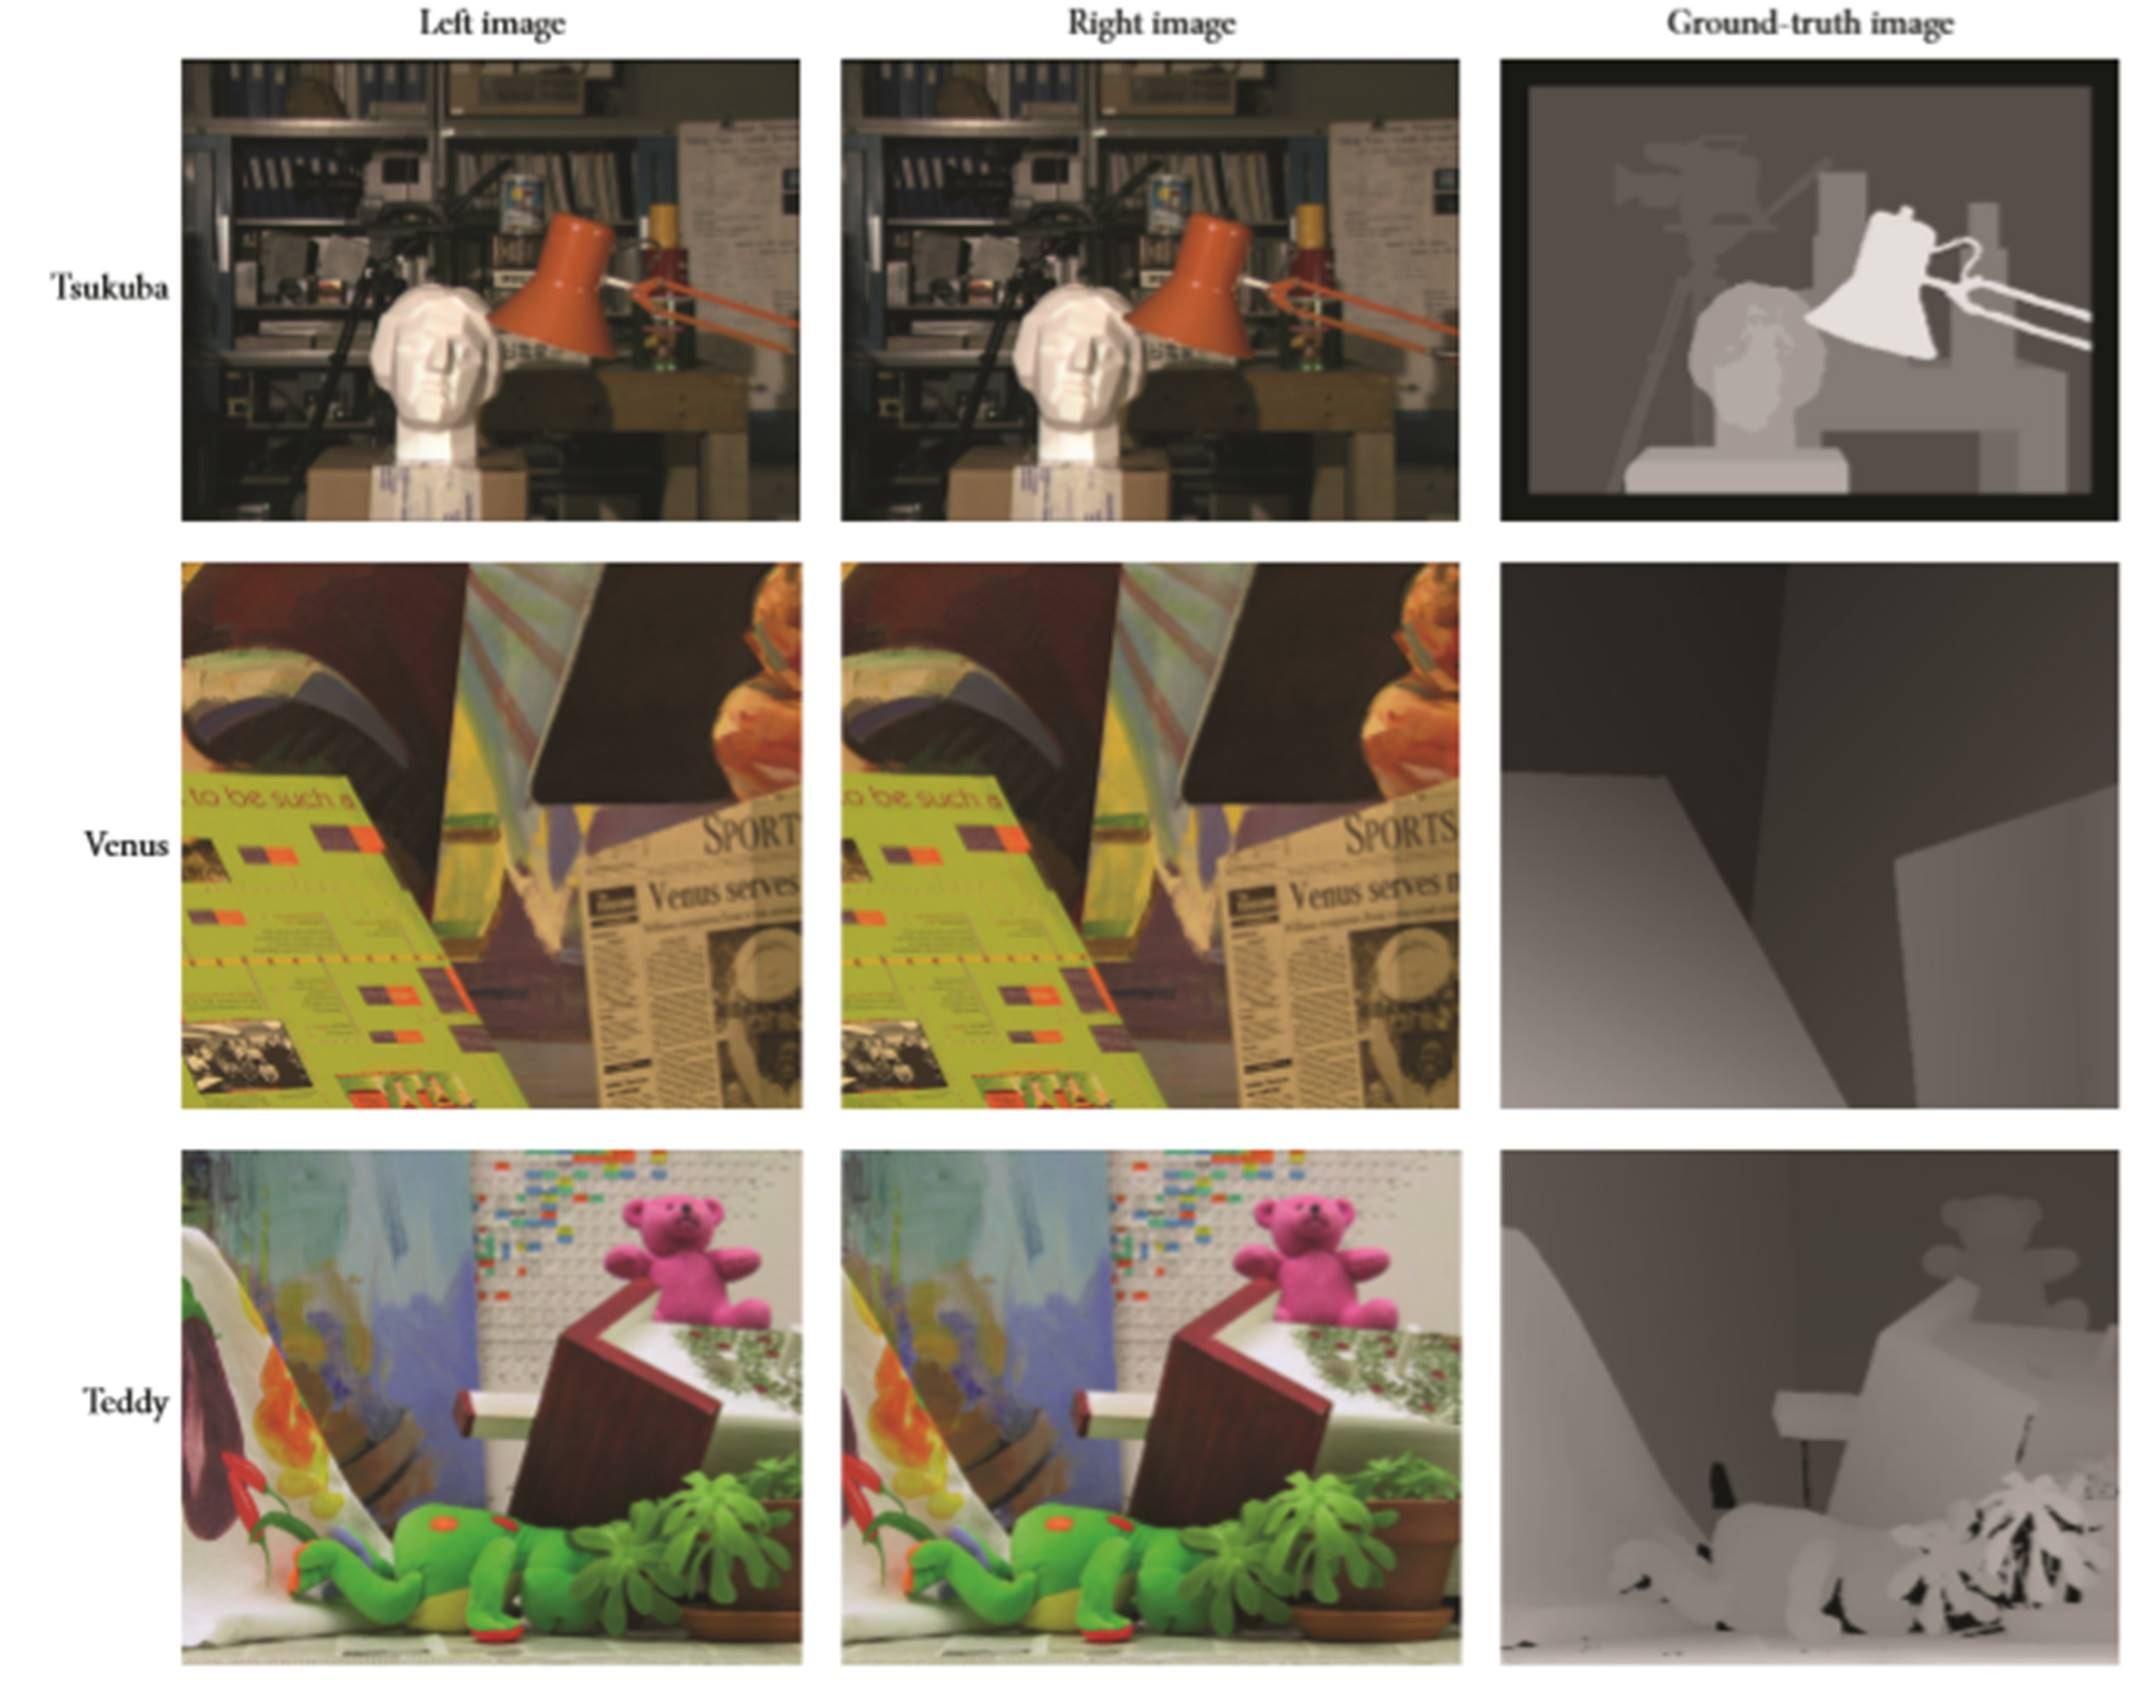
\includegraphics[width=9cm]{disparity_map.jpg}
    \end{center}
\end{frame}

\begin{frame}{Depth from disparity}
    \begin{columns}
        \column{0.5\textwidth}
        $x_L=f\frac{X}{Z}$ and $x_R=f\frac{X+T_x}{Z}$ implies
        $$Z=\frac{fT_x}{d}$$
        $T_x$ is base line and $d$ is disparity
        \column{0.5\textwidth}
        \begin{center}
            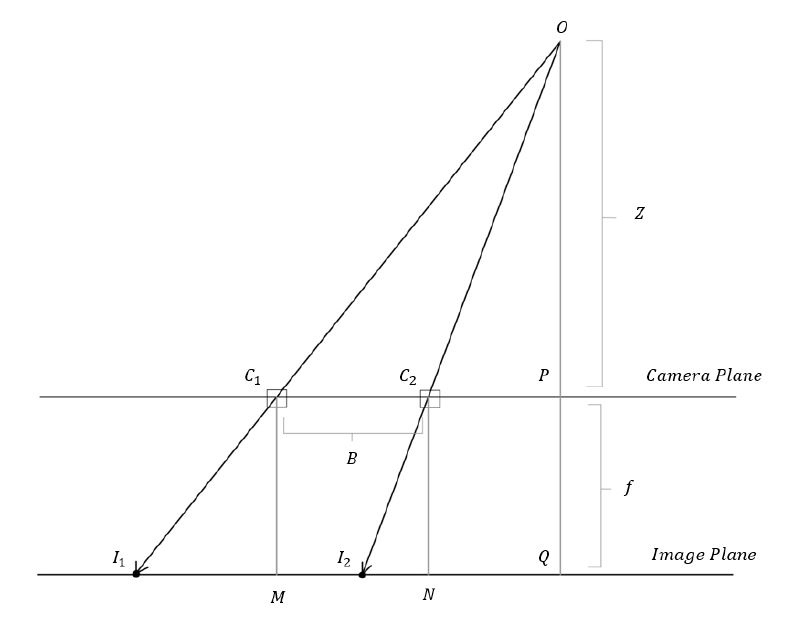
\includegraphics[width=6cm]{depth_from_disparity.JPG}
            \par Image from \cite{chaijirawiwat_monocular_2019}
        \end{center}
    \end{columns}
    
\end{frame}

\begin{frame}[allowframebreaks]
    \frametitle{References}
    \nocite{*}
    \bibliographystyle{unsrt}
    \bibliography{citations.bib}
\end{frame}

\end{document}